\documentclass[conference]{IEEEtran}
\IEEEoverridecommandlockouts

\usepackage{tikz}
\usepackage{parskip}

\usepackage{forest}
\usepackage{cite}
\usepackage{amsmath,amssymb,amsfonts}
\usepackage{algorithmic}
% \usepackage{graphicx}
\usepackage{textcomp}
\usepackage{xcolor}

\def\BibTeX{{\rm B\kern-.05em{\sc i\kern-.025em b}\kern-.08em
    T\kern-.1667em\lower.7ex\hbox{E}\kern-.125emX}}

\begin{document}

\title{Opponent Modelling in the Iterated Prisoner's Dilemma: A Literature Review}

\author{\IEEEauthorblockN{Faqih Mahardika}
\IEEEauthorblockA{\textit{Department of Computer Science and Electronics} \\
\textit{Gadjah Mada University} \\
Yogyakarta, Indonesia \\
fm.faqihmahardika@gmail.com}
}

\maketitle

\begin{abstract}

\end{abstract}

\begin{IEEEkeywords}
keyword1, keyword2, keyword3 
\end{IEEEkeywords}

\section{Introduction}
Cooperation and conflict are fundamental features of interaction in human societies, biological systems, and artificial-agent environments. Game theory offers a powerful analytical framework for studying such strategic interdependence, and seminal work on the evolution of cooperation has shown how behavioural patterns emerge when agents repeatedly face dilemmas that require balancing self-interest with mutual benefit\cite{axelrod_evolution_1981, axelrod_evolution_nodate}. Among these models, the Prisoner's Dilemma (PD) has become the canonical representation of situations in which individual rationality conflicts with collective welfare. In the one-shot PD, mutual cooperation yields the highest joint payoff, yet the incentives embedded in the payoff structure drive both players toward mutual defection, revealing a fundamental tension at the heart of many social, economic, and political interactions.

When this game is repeated over time as the Iterated Prisoner's Dilemma (IPD), the strategic landscape changes significantly. Repetition allows agents to condition their choices on one another's past actions, enabling behaviours such as reciprocity, retaliation, forgiveness, and trust-building. Axelrod's influential IPD tournaments demonstrated that simple contingent strategies most notably Tit-for-Tat could foster stable cooperation even in competitive environments, highlighting how long-term interaction and memory support the emergence of cooperative norms in the absence of central enforcement\cite{axelrod_evolution_nodate, axelrod_evolution_1981}.

The relevance of IPD dynamics extends far beyond abstract models. In biology, theories of reciprocal altruism describe how repeated encounters among organisms can favour contingent cooperation, laying out conditions under which helping behaviour can evolve among self-interested individuals\cite{trivers_evolution_1971}. Evolutionary game theory further formalises these mechanisms through the concept of evolutionarily stable strategies, demonstrating how certain behavioural rules can persist within populations under selective pressure\cite{smith_evolution_nodate}. Social and economic research similarly uses repeated-game frameworks to explain human cooperation, norm enforcement, and punishment in public-goods contexts\cite{charness_cooperation_2021}, while resource-management problems such as commercial fishing exemplify how strategic interdependence in shared environments mirrors the structure of repeated dilemmas\cite{leung_analysis_1976}. Across these domains, the IPD framework provides a versatile lens for understanding how cooperation can arise, stabilize, or collapse under varying incentives and institutional conditions.

Although classical analyses of the IPD provide essential foundations, their assumptions often diverge from the realities of strategic interaction. Real agents whether human, animal, or artificial frequently operate under uncertainty, face limited observability, and adapt their behaviour dynamically. Consequently, much of the recent literature emphasizes the need for models that allow agents to learn from experience and form expectations about others' behaviour over time. This motivates the development of opponent modelling, a set of techniques that enable one agent to infer an opponent's intentions, strategy, or behavioural tendencies based on observed actions. Contemporary surveys outline a wide spectrum of approaches to opponent modelling in adversarial and multi-agent settings, revealing that it plays a central role in enabling adaptive decision-making in repeated games, negotiation, autonomous control, and strategic competition\cite{nashed_survey_nodate}. In the context of the IPD, the ability to anticipate an opponent's future behaviour is especially critical: cooperation thrives when agents can recognise cooperative partners and detect exploiters, adjust to non-stationary strategies, and respond appropriately to shifts in interaction patterns.

By integrating insights from evolutionary theory, behavioural experimentation, and modern learning-based modelling, research on the IPD and opponent modelling provides a comprehensive view of how cooperation emerges and how strategic agents adapt to one another.\@ Yet findings across these fields remain fragmented, and a focused synthesis is needed to understand how opponent-modelling techniques have been conceptualised, implemented, and evaluated specifically within the IPD.\@ This literature review aims to address that gap by examining existing approaches, analysing their underlying assumptions, and identifying methodological challenges and research opportunities that shape the future of adaptive behaviour in repeated strategic environments.
\section{Related Work}
Your literature review and related work section.~\cite{axelrod_evolution_1981}


\section{Methodology}
Description of your methodology.
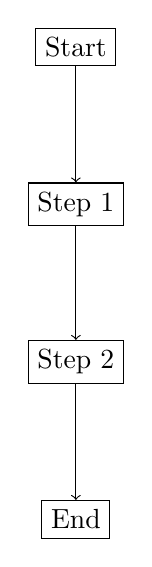
\begin{tikzpicture}
    \node (A) at (0,0) [draw, rectangle] {Start};
    \node (B) at (0,-2) [draw, rectangle] {Step 1};
    \node (C) at (0,-4) [draw, rectangle] {Step 2};
    \node (D) at (0,-6) [draw, rectangle] {End};

    \draw[->] (A) -- (B);
    \draw[->] (B) -- (C);
    \draw[->] (C) -- (D);
\end{tikzpicture}

\forestset{
  mynode/.style={
    draw,
    rounded corners,
    align=center,
    inner sep=4pt
  },
  header/.style={
    text width=2.8cm,
    inner sep=2pt,
    font=\bfseries
  },
  citation/.style={
    text width=2.8cm,
    inner sep=2pt,
    font=\footnotesize
  }
}

\begin{forest}
for tree={mynode}
[Root
    [Layer 1A
        [Child A1
            [ { \begin{tabular}{c}
                \textbf{Iterated Prisoner's Dilemma}\\
                \footnotesize\cite{axelrod_evolution_1981}
                \end{tabular} }
            ]
        ]
    ]
]
\end{forest}



\section{Results}
Your experimental results.

\section{Conclusion}
Your conclusions and future work.

\begin{thebibliography}{00}

\bibitem{nashed_survey_nodate}
S. B. Nashed and S. Zilberstein, ``A Survey on Opponent Modeling in Adversarial Domains,'' unpublished.

\bibitem{axelrod_evolution_nodate}
R. Axelrod, ``The Evolution of Cooperation'' unpublished.

\bibitem{axelrod_evolution_1981}
R. Axelrod and W. D. Hamilton, ``The Evolution of Cooperation'' \textit{Science}, 1981.

\bibitem{trivers_evolution_1971}
R. L. Trivers, ``The Evolution of Reciprocal Altruism'' \textit{The Quarterly Review of Biology}, vol. 46, no. 1, pp. 35--57, 1971.  
Available: https://www.journals.uchicago.edu/doi/10.1086/406755

\bibitem{charness_cooperation_2021}
Y. Chen, ``Cooperation and punishment in public goods experiments (by Ernst Fehr and Simon Gächter),'' in \textit{The Art of Experimental Economics}, G. Charness and M. Pingle, Eds., London: Routledge, 2021, pp. 134--143.  
Available: https://www.taylorfrancis.com/books/9781003019121/chapters/10.4324/9781003019121-12

\bibitem{leung_analysis_1976}
A. Leung and A.-Y. Wang, ``Analysis of Models for Commercial Fishing: Mathematical and Economical Aspects,'' \textit{Econometrica}, vol. 44, no. 2, p. 295, 1976.  
Available: https://www.jstor.org/stable/1912725

\bibitem{smith_evolution_nodate}
J. M. Smith, \textit{Evolution and the Theory of Games}. (Publication year not provided.)



\end{thebibliography}


\end{document}